\documentclass[12pt]{article}
\usepackage[a4paper,width=6.8in,height=8.8in]{geometry}
\usepackage{amsmath,amssymb}

\usepackage{amsmath,amssymb,mathtools,amsthm,
	textcomp,mathscinet}
\usepackage{listings}
\usepackage{amsfonts,graphicx,enumerate,subcaption,placeins}
\interdisplaylinepenalty=0
\usepackage[hidelinks]{hyperref}
\usepackage{setspace}
\usepackage[utf8]{inputenc}
\usepackage[english]{babel}
\usepackage{booktabs,multirow}
\usepackage{blkarray}
\usepackage{lscape}
\usepackage[T1]{fontenc}
\usepackage{authblk,color}
\usepackage[english]{babel}
\usepackage{amsfonts, amstext, amsthm, booktabs, dcolumn}
\usepackage{graphicx}
\usepackage{float}
\usepackage{caption}
\usepackage{centernot}
%\usepackage{subcaption}
\usepackage{times}
\usepackage[nottoc]{tocbibind}
\usepackage[mathscr]{eucal}
%\usepackage[numbers]{natbib}
%\usepackage{refcheck}
\usepackage[makeroom]{cancel}

\definecolor{gr}{rgb}{0.7, 0.0, 0.15}
\newcommand{\matindex}[1]{\mbox{\scriptsize#1}}
\newtheorem{proposition}{\bf Proposition}[section]
\newtheorem{theorem}{\bf Theorem}[section]
\newtheorem{cor}{\bf Corollaries}[section]
\newtheorem{corollary}{\bf Corollary}[section]
\newtheorem{remark}{\bf Remark}[section]
\newtheorem{remarks}{\bf Remarks}[section]
\newtheorem{lemma}{\bf Lemma}[section]
\newtheorem{definition}{\bf Definition}[section]
\newtheorem{example}{\bf Example}[section]
\newtheorem{results}{\bf Result}[section]
\def\thetheorem{\thesection.\arabic{theorem}}
\def\theremark{\thesection.\arabic{remark}}
\def\thecorollary{\thesection.\arabic{corollary}}
\def\thelemma{\thesection.\arabic{lemma}}
\newcommand\floor[1]{\left\lfloor#1\right\rfloor}
\newcommand\ceil[1]{\left\lceil#1\right\rceil}
\providecommand{\keywords}[1]{\textbf{\textit{Keywords:}} #1}
\newcommand\scalemath[2]{\scalebox{#1}{\mbox{\ensuremath{\displaystyle #2}}}}
\numberwithin{equation}{section}
\setstretch{1.1}
\usepackage{graphicx}
\graphicspath{ {./images/} }
\usepackage{xcolor}

\definecolor{codegreen}{rgb}{0,0.6,0}
\definecolor{codegray}{rgb}{0.5,0.5,0.5}
\definecolor{codepurple}{rgb}{0.58,0,0.82}
\definecolor{backcolour}{rgb}{0.95,0.95,0.92}

\lstdefinestyle{mystyle}{
	backgroundcolor=\color{backcolour},   
	commentstyle=\color{codegreen},
	keywordstyle=\color{magenta},
	numberstyle=\tiny\color{codegray},
	stringstyle=\color{codepurple},
	basicstyle=\ttfamily\footnotesize,
	breakatwhitespace=false,         
	breaklines=true,                 
	captionpos=b,                    
	keepspaces=true,                 
	numbers=left,                    
	numbersep=5pt,                  
	showspaces=false,                
	showstringspaces=false,
	showtabs=false,                  
	tabsize=2
}

\lstset{style=mystyle}

\begin{document}
	\begin{center}
		\Huge{\bf Exploratory Project}\\
		\Large{CSM 291}\\
		\vspace{1cm}
		on\\
		\vspace{1cm}
		\textbf{\Huge{Linear Regression - Predicting}}\\
		\textbf{\Huge{Insurance Prices}}\\
		\vspace{3cm}
		\Large{Submitted By}\\
		\vspace{1cm}
		\textbf{\Large{Mr. Shrey Gupta}}\\
		\Large{B.Tech. Student of Mathematics \& Computing }\\
		\large{IIT(BHU), Varanasi}
		\vspace{2cm}
		
		
\includegraphics[scale=2.5]{iitbhu.png}
	\end{center}
	\thispagestyle{empty}
	\cleardoublepage
\setcounter{page}{1}

	\newpage
\section{Introduction}\label{intro}
The most interesting topic in the modern era is Machine Learning. Machine learning is an application of artificial intelligence (AI) that provides systems the ability to automatically learn and improve from experience. There are many divisions of Machine Learning. One of the most important topic in Machine Learning is \textit{Linear Regression}. Linear Regression can be used to solve a variety of real-world problems like predicting the housing prices, predicting the sales for a particular year of a company among many others. Also, a supervised learning algorithm is an algorithm in which we give the algorithm some training data to learn from and then after training make the predictions. Linear regression is also a supervised learning algorithm in which we have to fit a function $f$ that maps our inputs $X$ to the corresponding function values $f(x)$. One such problem is as follows:\\
Suppose we are given the data of an insurance company which contains the charges they charge for their insurance for a person using the provided information by the person.
\begin{center}
	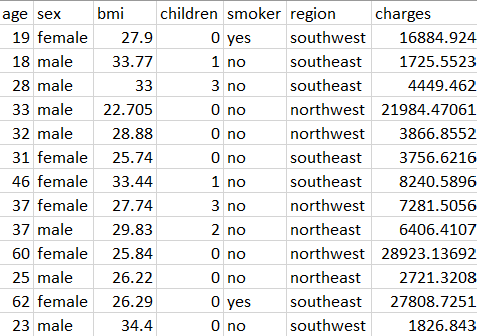
\includegraphics[height=8cm]{slide2}
\end{center}
Now, we wish to predict the insurance prices for a new person given his/her data.
We can do the above task by:
\begin{itemize}
	\item[(i)] Data Analysis
	\item[(ii)] Cleaning the data and preparing the dataset for training
	\item[(iii)] Make a model that best fits the data: Maximum Likelihood Estimation(MLE), Maximum a Posterior Estimation(MAP) and Bayesian Linear Regression(BLR).
	\item[(iv)] Make Predictions
\end{itemize}
In this project,  we  create a suitable model that will fit the training data well and make descent predictions based on the understandings from the literature survey.
\section{Literature Survey}\label{literature}
Regression is a supervised learning algorithm. In a regression problem, we have to fit a function $f$ that maps our inputs $X$ to the corresponding function values $f(x)$. For example,  suppose we are trying to predict the housing prices on the basis of the area (in sq. ft.) and we are given some training data for the same. We plot the graph for these training examples :- \\
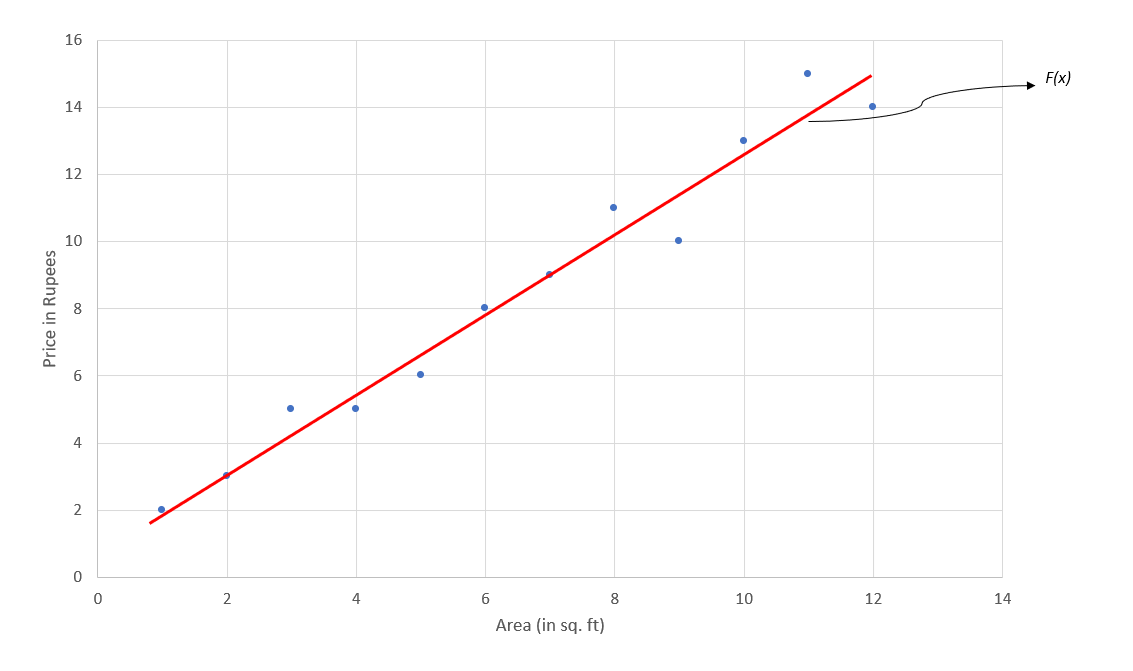
\includegraphics[width=\textwidth]{graph1}\\
We can clearly see that as the $area$ increases the $price$ also increases linearly. So, we can fit 
\begin{equation*}
	f(x)=\theta_{0} + \theta_{1}x
\end{equation*}
We have to determine these model parameters ($\theta_{0},\theta_{1}$) that fit this graph very well. Now, using this $f(x)$ we can predict house price given its area.\\
\textbf{The word``linear'' in linear regression means that the models that are ``linear in parameters'', that is, models that describe a function by a linear combination of input features, $X$.}\\
In the above example, let us assume that we are given set of training inputs, $x_{n}$ and corresponding noisy observations
$$y_{n}= f(x_{n}) + \epsilon,$$ 
where $\epsilon$ is the measurement noise. We assume $\epsilon$ is an independent and identically distributed random variable. It has a Normal (Gaussian) distribution with mean 0 and variance $\sigma^2$.
\begin{equation*}
	\epsilon \sim \mathcal{N}(0,\sigma^2)
\end{equation*}
\begin{center}
	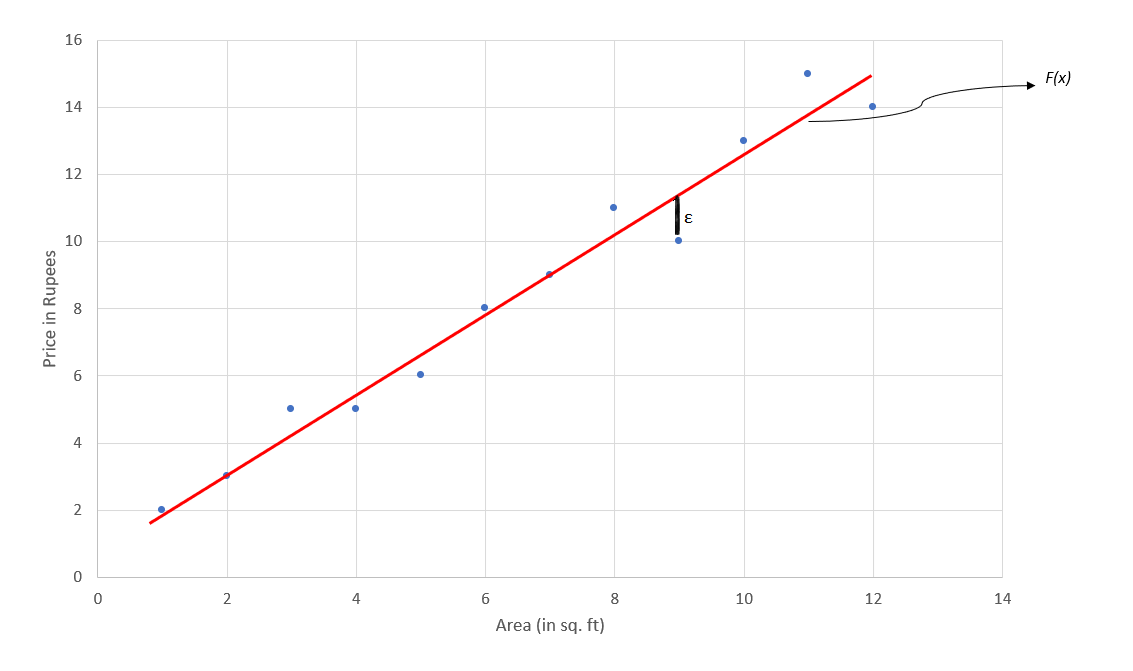
\includegraphics[width=10cm, height=10cm]{graph2}
\end{center}
So, finally our task in linear regression is to find a function that not only models the training data, but generalizes well to predicting function values at input locations that are not a part of the training set.
\subsection{Problem Formulation}
Let us consider the likelihood function
\begin{equation*}
	p(y|x)= \mathcal{N}(y|f(x),\sigma^2)
\end{equation*}
where $x \in \mathbb{R}^D$ are the inputs and $y \in \mathbb{R}$ are the targets. Here, $D$ refers to the number of features. Also, $y= f(x) + \epsilon$, where $\epsilon \sim \mathcal{N}(0,\sigma^2)$ is an independent and identically distibuted random variable that represents the noise. Suppose the graph for the training examples is as follows:
\begin{center}
	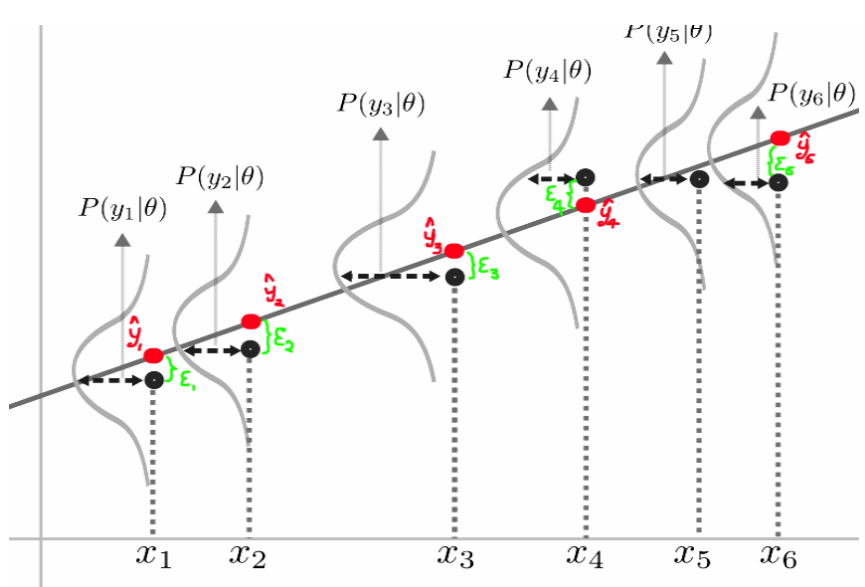
\includegraphics[width=10cm, height=10cm]{graph3}
\end{center}
For $y_{n}$ the mean of the distribution is $f(x_{n})$ and variance is $\sigma^2$. Now, for linear regression, we consider
\begin{equation*}
	f(x)=x^T\theta
\end{equation*}
where $x$ is the feature vector and $\theta$ is the model parameters vector. For example, consider that we are having $4$ features, then
\begin{align*}
	x&=\begin{bmatrix}
		x^{(1)}\\
		x^{(2)}\\
		x^{(3)}\\
		x^{(4)}\\
	\end{bmatrix}
\hspace{2cm}	\theta=\begin{bmatrix}
		\theta_{1}\\
		\theta_{2}\\
		\theta_{3}\\
		\theta_{4}\\
	\end{bmatrix}\\
f(x)&=x^T\theta\\
f(x)&=\begin{bmatrix}
	x^{(1)} & x^{(2)} & x^{(3)} & x^{(4)}
\end{bmatrix}
\begin{bmatrix}
	\theta_{1}\\
	\theta_{2}\\
	\theta_{3}\\
	\theta_{4}\\
\end{bmatrix}\\
f(x)&= x^{(1)}\theta_{1} + x^{(2)}\theta_{2} + x^{(3)}\theta_{3} + x^{(4)}\theta_{4}
\end{align*}\\
For the time being we assume $\sigma^2$ to be known. Hence, 	$p(y|x)= \mathcal{N}(y|x^T\theta,\sigma^2)$ $\Leftrightarrow$ $y = x^T\theta + \epsilon$, $\epsilon \sim \mathcal{N}(0,\sigma^2)$, where $\theta \in \mathbb{R}^D$ are the model parameters which we need to determine. Here, the likelihood is the probability density function of $y$ evaluated at $x^T\theta$.
\subsection{Parameter Estimitation}
Consider the training set,
\begin{equation*}
	Z=\{(x_{1},y_{1}), (x_{2},y_{2}), \dots, (x_{n},y_{n})\}
\end{equation*}
consisting of $N$ inputs $x_{n} \in \mathbb{R}^D$ and targets $y_{n} \in \mathbb{R}$, $n=1, 2, \dots, N$. Now, 
$$p(Y|X,\theta) = p(y_{1}, y_{2},\dots, y_{n}|x_{1}, x_{2}, \dots, x_{n}, \theta).$$
As we know that $y_{i}$ and $y_{j}$ are conditionally independent given their respective inputs $x_{i}$ and $x_{j}$. Therefore,
\begin{align*}
p(Y|X,\theta)&=\prod_{n=1}^{N} p(y_{n}|x_{n}, \theta)=\prod_{n=1}^{N} \mathcal{N}(y_{n}|x_{n}, \theta)
\end{align*}
where $X = \{x_{1}, x_{2}, \dots, x_{n}\}$ is the input set and $y = \{y_{1}, y_{2}, \dots, y_{n}\}$ is the target set. Now, we have to find optimal parameters $\theta^{*} \in \mathbb{R}^D$, so that they fit the data very well. Once we are able to find $\theta^{*}$ then we can predict function values using $y = x^T\theta + \epsilon$, so that at an arbitrary test input $x_{*}$ the distribution of the corresponding target $y_{*}$ is
\begin{equation*}
	p(y_{*}|x_{*, \theta^{*}})=\mathcal{N}(y_{*}|x_{*}^T\theta^*, \sigma^2).
\end{equation*}
\subsection{Maximum Likelihood Estimation}
Maximizing the likelihood means maximizing the predictive distribution of the training data given the model parameters. Mathematically, we have to evaluate
\begin{equation*}
	\theta_{ML} = \underset{\theta}{\arg\max}  P(Y|X,\theta).
\end{equation*}
We can find $\theta_{ML}$ by using an iterative approach called gradient descend on the negative likelihood. But there is a closed form solution for this, so gradient descend becomes unnecessary. In practice, instead of maximizing the likelihood directly, we apply the log-transformation to the likelihood function and then minimize the negative log-likelihood.

\vskip 1ex
\noindent
\textbf{Advantages of the log Likelihood}:
\begin{enumerate}
	\item It does not suffer from numerical underflow. As likelihood is the product of $N$ Gaussian distributions. Hence, multiplying $N$ probabilities can lead to very small number which can cause underflow.
	\item Differentiation becomes easier. Applying repeated product rule is very cumbersome. Rather in log-transformation we have sum of individual derivatives.
\end{enumerate}
Now,
\begin{align*}
	-\log p(Y|X,\theta)&=-\log\prod_{n=1}^{N}p(y_{n}|x_{n}, \theta)=-\sum_{n=1}^{N}\log p(y_{n}|x_{n}, \theta)
\end{align*}
We have to minimize this negative log-likelihood.
\begin{align*}
	p(y_{n}|x_{n}, \theta) &= \mathcal{N}(y_{n}|x_{n}^T\theta, \sigma^2)=\frac{e^{\frac{-(y_{n}-x_{n}^T\theta)^2}{2\sigma^2}}}{\sqrt{2\pi}\sigma}
	\end{align*}
	This implies
	\begin{align*}
	\log p(y_{n}|x_{n}, \theta)&= \log (\frac{1}{\sqrt{2\pi}\sigma}) - \frac{(y_{n}-x_{n}^T\theta)^2}{2\sigma^2}
\end{align*}
Ignoring the $\log (\frac{1}{\sqrt{2\pi}\sigma})$ (independent term of $\theta$), we have
\begin{align*}
	-\log p(y_{n}|x_{n}, \theta) = \frac{(y_{n}-x_{n}^T\theta)^2}{2\sigma^2}\\
\end{align*}
Now,
\begin{align}
		-\log p(Y|X, \theta) = \sum_{n=1}^{N} \frac{(y_{n}-x_{n}^T\theta)^2}{2\sigma^2}. \label{mle}
\end{align}
The negative log likelihood is also called \textit{Loss function}.
\begin{align*}
	\mathcal{L}(\theta) &= \frac{\sum_{n=1}^{N}(y_{n}-x_{n}^T\theta)^2}{2\sigma^2}=\frac{(y-X\theta)^T(y-X\theta)}{2\sigma^2} 
\end{align*}
where, 
\begin{align*}
	X=\begin{bmatrix}
		x_{1}^{(1)} & x_{1}^{(2)} & \dots & x_{1}^{(D)}\\
		x_{2}^{(1)} & x_{2}^{(2)} & \dots & x_{2}^{(D)}\\
		. & . & .& .\\
		. & . & .& .\\
		. & . & .& .\\
		x_{N}^{(1)} & x_{N}^{(2)} & \dots & x_{N}^{(D)}
	\end{bmatrix} \in \mathbb{R}^{NXD}
\end{align*}
is the feature matrix consisting of $N$ training inputs and $D$ features.
$$y = \begin{bmatrix}
	y_{1}\\
	y_{2}\\
	.\\
	.\\
	.\\
	y_{n}
\end{bmatrix} \in \mathbb{R}^N \text{ and } 
\theta = \begin{bmatrix}
	\theta_{1}\\
	\theta_{2}\\
	.\\
	.\\
	.\\
	\theta_{D}
\end{bmatrix} \in \mathbb{R}^D.$$
We see that the loss function is the sum of squared errors between $y_{n}$ and model prediction $x_{n}^T\theta$.
\begin{align*}
	\mathcal{L}&=\frac{(y-X\theta)^T(y-X\theta)}{2\sigma^2}=\frac{\|y-X\theta\|^2}{2\sigma^2}
\end{align*}
where $\|y-X\theta\| = (y-X\theta)^T(y-X\theta)$ and is called 2-norm of the matrix. Now, we need to find the global optimum of this function.
\begin{align*}
	\frac{\partial \mathcal{L}}{\partial \theta}&=\frac{\partial}{\partial \theta}(\frac{(y-X\theta)^T(y-X\theta)}{2\sigma^2})\\
	&=\frac{1}{2\sigma^2}\frac{\partial}{\partial \theta}((y^T - \theta^TX^T)(y - X\theta))\\
	&=\frac{1}{2\sigma^2}\frac{\partial}{\partial \theta}(y^{T}y-y^{T}X\theta-\theta^{T}X^{T}y+\theta^{T}X^{T}X\theta)
\end{align*}
We see that $y^TX\theta$ is a $1X1$ matrix and hence symmetric. Therefore, $y^TX\theta = (y^TX\theta)^T = \theta^TX^Ty$
\begin{align}\label{mle1}
	\frac{\partial \mathcal{L}}{\partial \theta}&=\frac{1}{2\sigma^2}\frac{\partial}{\partial \theta}(y^Ty - 2y^TX\theta + \theta^TX^TX\theta)\\ \nonumber
	&=\frac{1}{2\sigma^2}(0 - 2y^TX + 2\theta^TX^TX)\\ \nonumber
	&=\frac{1}{\sigma^2}(\theta^TX^TX - y^TX) 
\end{align}
Setting gradient to $0^T$ is a necessary and sufficient condition, and we will obtain the global optimum as Hessian $\nabla_{\theta}^2\mathcal{L}(\theta) = X^TX \in \mathbb{R}^{DXD}$.(Till $X^TX$ is positive and definite). Therefore,
\begin{align*}
	&\therefore \frac{\partial\mathcal{L}}{\partial\theta} = 0^T
	\end{align*}
	This implies
	\begin{align*}
 \theta_{ML}^TX^TX &= y^TX\\
	&\theta_{ML}^T = y^TX(X^TX)^{-1}\\
	&\theta_{ML} = (X^TX)^{-1}X^Ty .
\end{align*}
For all this to happen rank($X$) has to be equal to D. Because if rank($X$)=D.\\
$X^TX$ will be positive definite and invertible. Hence, Hessian will be positive and definite and will  have global optimum.

\subsection{Maximum Likelihood with Features}
Assume that we are given a dataset with the following graph
\begin{center}
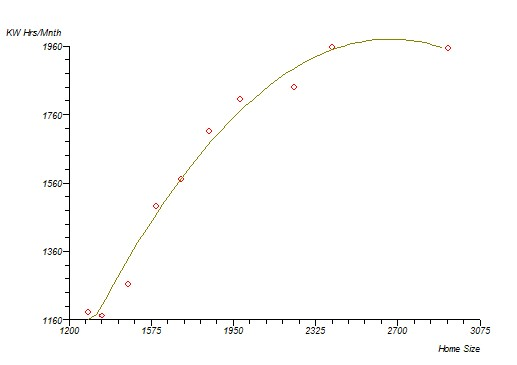
\includegraphics[width=15cm, height=5cm]{graph4}
\end{center}
We can clearly see that a straight line will not fit this data. Instead we need a polynomial fit for this data. Since linear regression only refers to linear in parameters, we can perform an arbitrary non-linear transformation $\phi(x)$ of the inputs $x$ and then linearly combine the components of this transformation. Therefore,
\begin{align*}
p(y|x,\theta) = \mathcal{N}(y|\phi^T(x)\theta, \sigma^2)\Leftrightarrow y = \phi^T(x)\theta + \epsilon = \sum_{k=0}^{K-1}\theta_{k}\phi_{k}(x) +\epsilon
\end{align*}
where $\phi$ : $\mathbb{R}^D \rightarrow \mathbb{R}^K$ is a non linear transformation of inputs $x$. $\phi_{k}$ : $\mathbb{R}^D \rightarrow \mathbb{R}$ is the $k$th component of the vector $\phi$. For example,
\begin{equation*}
	\phi(x) = \begin{bmatrix}
		1\\ x\\ x^2\\ .\\ .\\ .\\ x^{K-1}
	\end{bmatrix}
= \begin{bmatrix}
	\phi_{0}(x)\\ \phi_{1}(x)\\ \phi_{2}(x)\\ .\\ .\\ .\\ \phi_{K-1}(x)
\end{bmatrix} \in \mathbb{R}^K
\end{equation*}
So in simple words we have increased the number of features from 1 to $K$. Now, generalizing the things. The design(feature) matrix will be:
\begin{equation*}
	\Phi = \begin{bmatrix}
		\phi^T(x_{1})\\ \phi^T(x_{2})\\ .\\ .\\ .\\ \phi^T(x_{N}) 
	\end{bmatrix}
= \begin{bmatrix}
	\phi_{0}(x_{1})& \phi_{1}(x_{1})& .& .& .& \phi_{K-1}(x_{1})\\
	\phi_{0}(x_{2})& \phi_{1}(x_{2})& .& .& .& \phi_{K-1}(x_{2})\\
	.& .& .& .& .& .&\\ 
	.& .& .& .& .& .&\\
	.& .& .& .& .& .&\\
	\phi_{0}(x_{N})& \phi_{1}(x_{N})& .& .& .& \phi_{K-1}(x_{N})
\end{bmatrix}
\end{equation*}
where $x_{n} \in \mathbb{R}^D$ are the training inputs and $y_{n} \in \mathbb{R}$ are the targets, $n=1, 2, 3, \dots, N.$ The model parameters 
$$\theta = \begin{bmatrix}
	\theta_{0}\\ \theta_{1}\\ \theta_{2}\\ .\\ .\\ .\\ \theta_{K-1}
\end{bmatrix} \in \mathbb{R}^K.$$
For example. For third order polynomials. Assume $x_{n} \in \mathbb{R}, n=1, 2, \dots, N$ be the inputs and $y_{n} \in \mathbb{R}$ be the targets. Then, 
$$\Phi = \begin{bmatrix}
	1 & x_{1} & x_{1}^2 & x_{1}^3\\
	1 & x_{2} & x_{2}^2 & x_{2}^3\\
	1 & x_{3} & x_{3}^2 & x_{3}^3\\
	. & . & . & .\\
	. & . & . & .\\
	. & . & . & .\\
	1 & x_{N} & x_{N}^2 & x_{N}^3
\end{bmatrix} \in \mathbb{R}^{NX4} \hspace{1cm}
\text{and} \hspace{1cm} \theta = \begin{bmatrix}
	\theta_{0}\\ \theta_{1}\\ \theta_{2}\\ \theta_{3}
\end{bmatrix} \in \mathbb{R}^4$${Now combining it with our normal likelihood we see that we have only changed $X$ with $\Phi$. Hence,
\begin{equation*}
	\theta_{ML} = (\Phi^T\Phi)^{-1}\Phi^Ty.
\end{equation*}
Here, $\Phi^T\Phi$ is invertible if rank$(\Phi)$ is $K$.


\subsection{Estimating Noise Variance}
Till now we have assumed that $\sigma^2$ was known to us. But we can calculate $\sigma_{ML}^2$ for noise variance with the help of likelihood function. Now
\begin{align*}
\hspace{1cm}  \log p(Y|X, \theta, \sigma^2) &= \sum_{n=1}^{N}\log \mathcal{N}(y_{n}| \phi^T(x_{n})\theta, \sigma^2)\\
	&= \sum_{n=1}^{N} (\frac{-\log(2\pi)}{2} - \frac{\log \sigma^2}{2} - \frac{(y_{n}-\phi^T(x)\theta)^2}{2\sigma^2})\\
	&= -\frac{N}{2}\log \sigma^2 - \frac{\sum_{n=1}^{N}(y_{n}-\phi^T(x_{n})\theta)^2}{2\sigma^2} + const
\end{align*}
Assuming $\sigma^2 = z$ and $\sum_{n=1}^{N}(y_{n}-\phi^T(x_{n})\theta)^2 = S$
\begin{equation*}
	\log p(Y|X, \theta, \sigma^2) = -\frac{N}{2}\log z - \frac{S}{2z} + \text{constant}.
\end{equation*}
Now partial derivative $w.r.t.$ z.
\begin{equation*}
	\frac{\partial}{\partial z}\log p(Y|X, \theta, \sigma^2) = -\frac{N}{2z} + \frac{S}{2z^2}
\end{equation*}
Now putting this derivative to 0.
\begin{align*}
	-\frac{N}{2z} + \frac{S}{2z^2} &= 0\implies z = \frac{S}{N}
\end{align*}
Therefore,
\begin{equation*}
 \sigma_{ML}^2 = \frac{\sum_{n=1}^{N}(y_{n}-\phi^T(x_{n})\theta)^2}{N}.
\end{equation*}
\subsection{Overfitting in Linear Regression} \label{overfitting}
We can see that even after fitting the best possible curve for the dataset we still have some error in the model. We can evaluate the quality of the model by:
\begin{enumerate}
	\item The Negative Log-Likelihood
	\begin{equation*}
		\mathcal{L}(\theta_{ML}) = \frac{(y-X\theta_{ML})^T(y-X\theta_{ML})}{2\sigma^2}
	\end{equation*}
	Less the loss better the model.
	\item Using RMSE
	\begin{equation*}
		RMSE = \sqrt{\frac{\sum_{n=1}^{N}(y_{n}- \phi^T(x_{n})\theta)^2}{N}}
	\end{equation*}
	less the loss better the model.
\end{enumerate}
So by these two ways we can evaluate the quality of our model. Let us assume that we have determined the best degree of the polynomial by finding the polynomial degree M that minimizes the loss function or RMSE. If we assume that the polynomial degree is a natural number, we can perform brute-force search and enumerate all the reasonable values of M.\\
For a training set of size $N$ it is sufficient to test $0 \le M \le N-1$. Because for $M \ge N$ we will have more parameters($\theta$) than the data points, that will lead to $\Phi^T\Phi$ being non-invertible, so that there will be infinite many possible maximum likelihood parameters($\theta_{ML}$). Suppose that we plot the graphs with different values of $M$ with $N = 10$ training examples.

\noindent
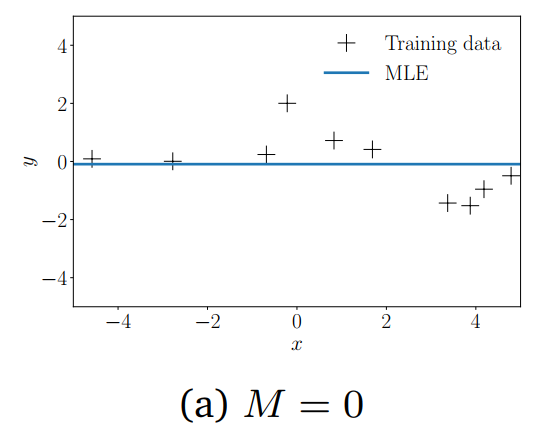
\includegraphics[scale=0.48]{graph5} 
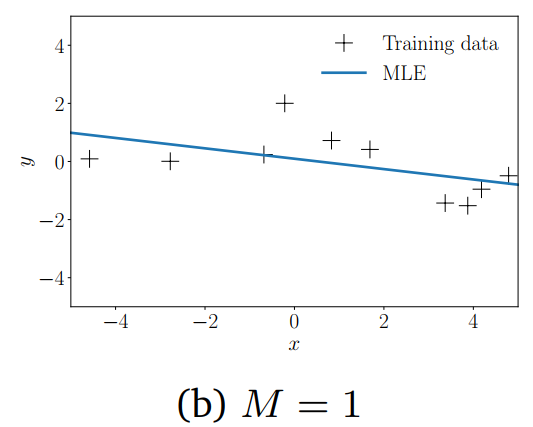
\includegraphics[scale=0.48]{graph6}
 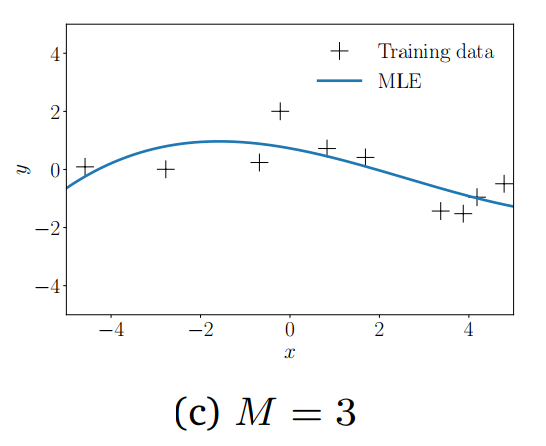
\includegraphics[scale=0.48]{graph7}\\
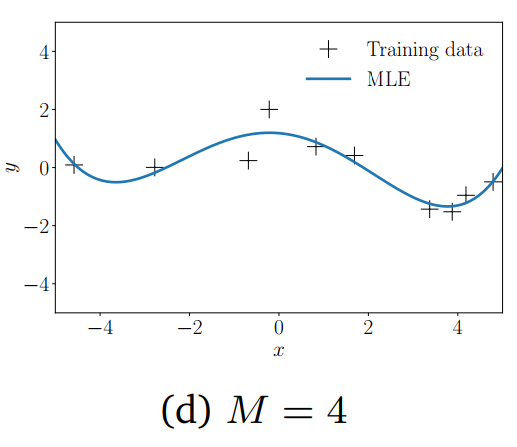
\includegraphics[scale=0.48]{graph8} 
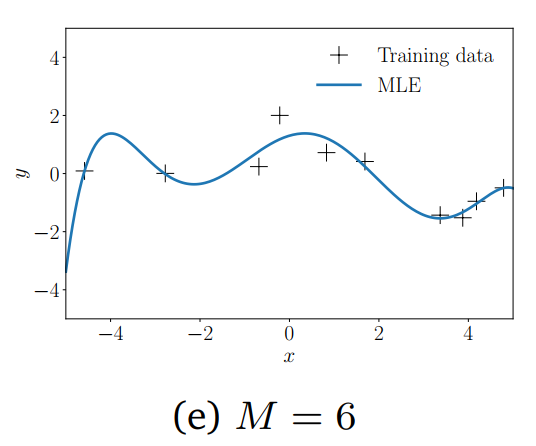
\includegraphics[scale=0.48]{graph9} 
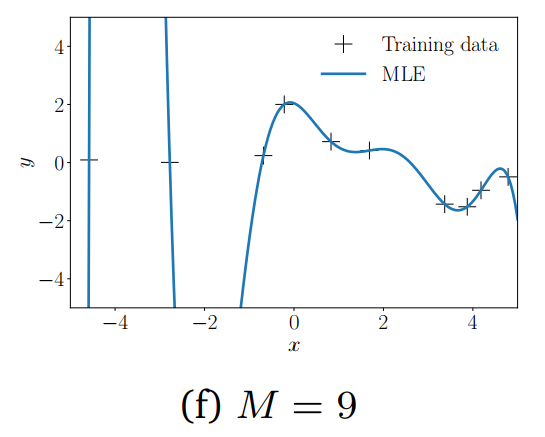
\includegraphics[scale=0.48]{graph10}\\
We clearly see that for low degree polynomials($M= 0, 1$) the curve fit the data poorly. This is called underfitting. For $M= 3-5$, the curve was reasonably fitting the data good.\\
Bur for $M= 9$, we see that the curve fit the data points very correctly without leaving any point. This is known as overfitting. It we analyse the graph for $M= 9$, we will see that if we will provide a new test data point to our model then it will predict rubbish values as the graph is sometimes overshooting and is not that much stable. But as we know that our prime objective of linear regression is to predict correct values for unseen data points. But our model for high degree polynomials though fit the training data into account but does not generalizes the result. So, to check our model performance, we have to take into account both the training error and test error. We can split our data set into two parts
\begin{enumerate}
	\item Training Set - For training the model
	\item Test/Dev Set - For testing our model
\end{enumerate}
For example -  For the above graphs if we plot a graph between \textit{Degree of polynomial Vs RMSE}.
\begin{center}
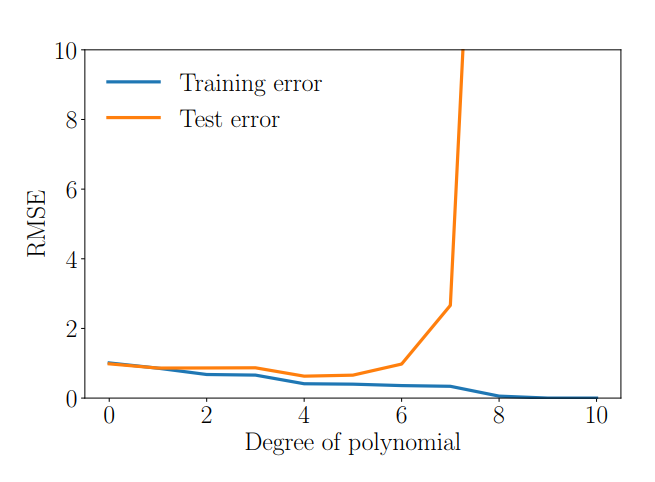
\includegraphics[width=\columnwidth/2]{graph11}
\end{center}
So we see that $M=4$ generalizes test data well as well as fits the training data well.

\subsection{Maximum A Posteriori Estimation}
We know that MLE(Maximum Likelihood Estimation) is prone to overfitting.\\
Also it is observed that when we run into overfitting then our parameters($\theta$) becomes relatively large.\\
So we can reduce overfitting by making our parameters values not too large. We can achieve this by placing a prior distribution $p(\theta)$ on the parameters.\\
\textbf{Example} Consider a Gaussian prior $p(\theta) = \mathcal{N}(0, 1)$. Therefore,
\begin{align*}
e p(\theta) &= \frac{e^{\frac{-\theta^2}{2}}}{\sqrt{2\pi}}.
\end{align*}
\begin{center}
	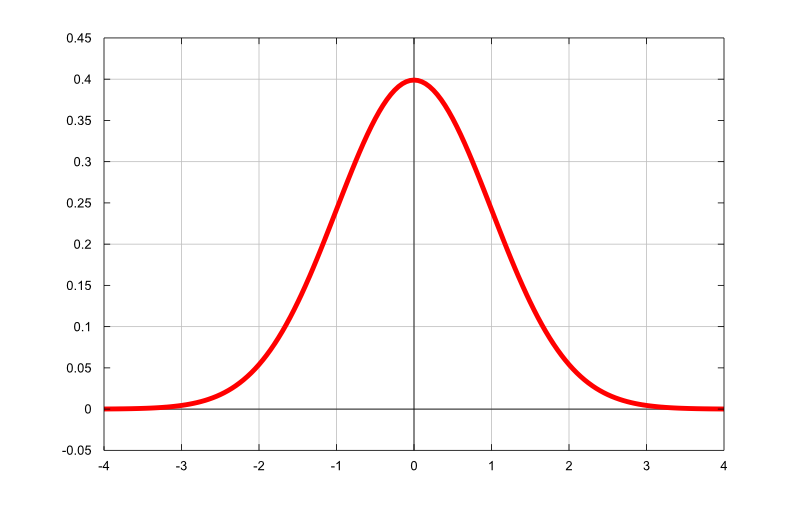
\includegraphics[width=\columnwidth/2, height=5cm]{graph12}
\end{center}
We see that here probability of $\theta$ is maxed around $0$, and $\theta$ is expected to lie in $[-2, 2]$ (two standard deviations around mean). Given our training data $X, Y$. Here we will maximize the posterior distribution $p(\theta|X, Y)$. This method is called maximum a posterior(MAP) estimation. Now, applying Baye's theorem, we get
\begin{equation}
	p(\theta|X, Y) = \frac{p(Y|X, \theta)p(\theta)}{p(Y|X)} \label{bayes}
\end{equation}
Now we have to find $\theta_{MAP}$ that maximizes the $p(\theta|X, Y)$. Applying log to equation \eqref{bayes}
\begin{equation*}
	\log p(\theta|X, Y) = \log p(Y|X, \theta) + \log p(\theta) - \log p(Y|X)
\end{equation*}
Here, $p(Y|X)$ is independent of $\theta$. Hence, 
\begin{equation}
	\log p(\theta|X, Y) =  \log p(Y|X, \theta) + \log p(\theta) + const \label{map1}
\end{equation}
We see that \textit{log posterior} is the sum of \textit{log- likelihood} $p(Y|X, \theta)$ and \textit{log-prior}. Hence MAP estimate will be a compromise between prior and likelihood. Now, $\theta_{MAP} \in \underset{\theta}{\arg\max}(-\log p(Y|X, \theta) - \log p(\theta))$. We assume that $p(\theta) = \mathcal{N}(0, b^2I)$. Here, $I$ is the identity matrix, which is used for maintaining correct dimensions of the equations. Using equations \eqref{map1} and \eqref{mle}, we have
\begin{align*}
	-\log p(\theta|X, Y) = \frac{(y-\Phi\theta)^T(y-\Phi\theta)}{2\sigma^2} + \frac{\theta^T\theta}{2b^2} + const
\end{align*}
Using equation \eqref{mle1}
\begin{equation*}
	\frac{-\partial \log p(\theta|X, Y)}{\partial \theta} = \frac{(\theta^T\Phi^T\Phi - y^T\Phi)}{\sigma^2} + \frac{\theta^T}{b^2}
\end{equation*}
Now putting it to $0^T$.
\begin{flalign*}
	&&\frac{(\theta^T\Phi^T\Phi - y^T\Phi)}{\sigma^2} + \frac{\theta^T}{b^2} &= 0^T&\\
	&\implies &\theta^T(\frac{\Phi^T\Phi}{\sigma^2}+ \frac{I}{b^2}) - \frac{y^T\Phi}{\sigma^2} &= 0^T&\\
	&\implies &\theta^T(\Phi^T\Phi + \frac{\sigma^2}{b^2}I) &= y^T\Phi&\\
	&\implies &\theta^T &= y^T\Phi(\Phi^T\Phi + \frac{\sigma^2}{b^2}I)^{-1}&\\
	&\implies &\theta_{MAP} &= (\Phi^T\Phi + \frac{\sigma^2}{b^2}I)^{-1}\Phi^Ty&
\end{flalign*}
So comparing this with MLE we see that the only change is the addition of $\frac{\sigma^2}{b^2}I$ term in the inverse matrix. This term $\frac{\sigma^2}{b^2}I$ ensures that $\Phi^T\Phi + \frac{\sigma^2}{b^2}I$ is symmetric and strictly positive definite. Hence, its inverse always exist. Also, it represents the impact of regularization which prevents $\theta$ from taking too large values.

\noindent
\textbf{Example}. Consider the graphs which we analyzed in section \ref{overfitting} Overfitting in MLE. But now let us define a prior $p(\theta) = \mathcal{N}(0, I)$.\\
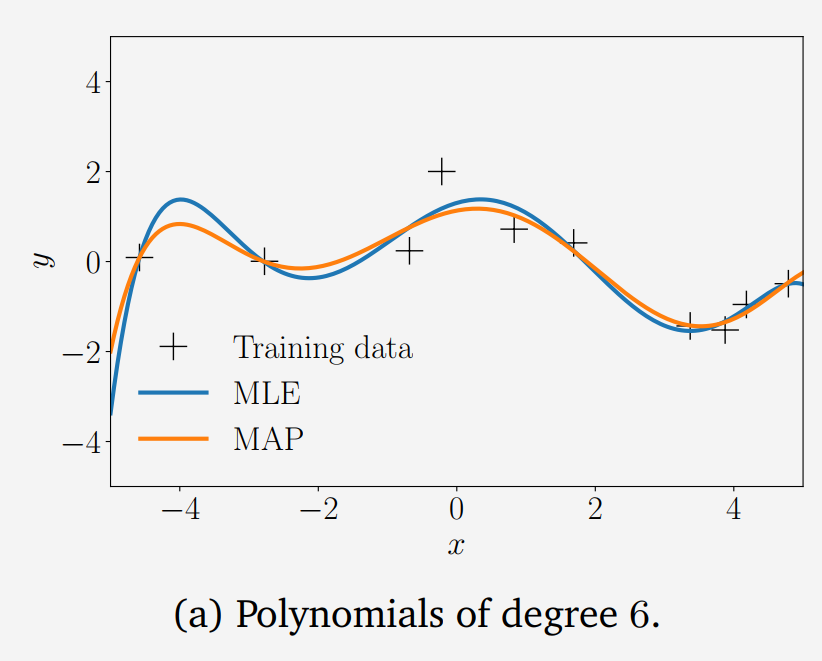
\includegraphics[scale=0.48]{garph13} 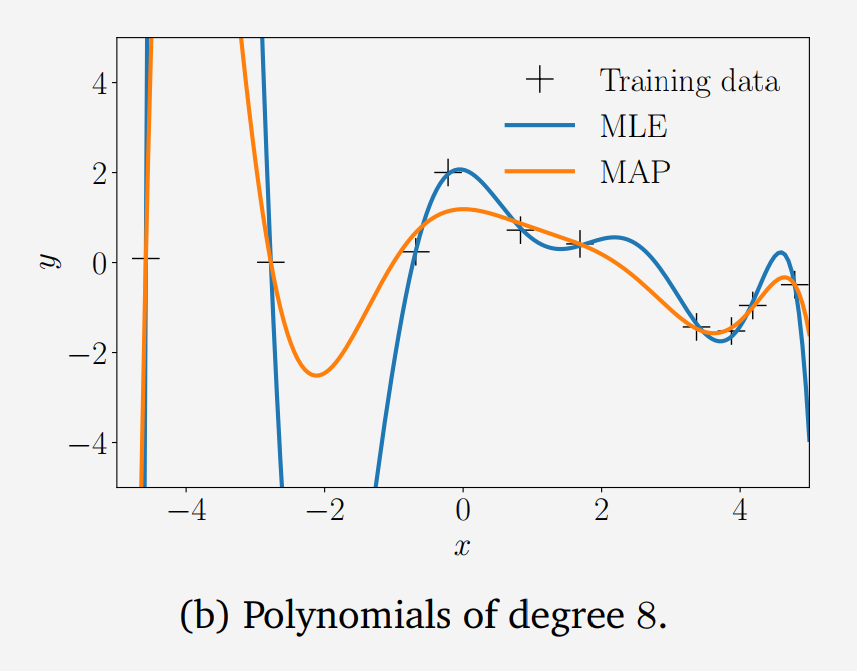
\includegraphics[scale=0.48]{graph14} \\
We see that for lower degree of polynomial, MAP estimate does not played a significant role. We see for high degree polynomials MAP kept the function relatively smoother and prevented overfitting to some extent.


\subsection{MAP Estimation as Regularization}
We can prevent overfitting by a method called regularization. In this method, our loss function is 
\begin{equation*}
	\mathcal{L}(\theta) = \|y - \Phi\theta\|^{2} + \lambda \|\theta\|_{2}^2 \hspace{1cm} (\|\theta\|_2^2 = \sum\theta^2_{i})
\end{equation*}
where $\|.\|$ is the euclidean norm and $\lambda$ is regularization constant. $\lambda \in [0, \infty)$. This parameter decides to what extent we have to do regularization. More $\lambda$ more regularization. As we know that we want to minimize $\mathcal{L}(\theta)$ hence this $\lambda \|\theta\|_2^2$ will prevent $\theta_{i}'s$ to be large. Hence preventing overfitting. Now comparing $\lambda \|\theta\|_2^2$ with negative log prior = $\frac{\|\theta\|_2^2}{2b^2} + const$. We can say that $\lambda = \frac{1}{2b^2}$. We see that here $\mathcal{L}(\theta)$ is very much identical to the MAP estimate. Hence, 
\begin{equation*}
	\theta_{RLS} = (\Phi^T\Phi + \lambda I)^{-1}\Phi^Ty
\end{equation*}
For $\lambda = \frac{\sigma^2}{b^2}$, this is identical to MAP estimate.
\subsection{Bayesian Linear Regression}
Bayesian linear regression does not attempt to compute a point estimate of the parameters, but instead the full posterior distribution over parameters($\theta$) is taken into account when making predictions. This means we compute the mean over all plausible parameter settings.

\noindent
For Bayesian linear regression, consider,\\
\textbf{prior} $p(\theta) = \mathcal{N}(m_o, S_o)$\\
\textbf{likelihood} $p(y|x, \theta) = \mathcal{N}(y|\phi^T(x)\theta. \sigma^2)$,\\
which is somewhat very similar to the MAP estimate except the prior.

\subsubsection{Prior Predictions}
In this method, we take the parameters($\theta$) and average over all the plausible parameter settings when we make predictions.
\begin{align*}
	 p(y_*|x_*) &= \int p(y_*|x_*, \theta)p(\theta)d\theta\\
	 &= E_\theta[p(y_*|x_*, \theta)]
\end{align*}
We see that this is an average prediction of $p(y_*|x_*, \theta)$ for all the plausible values of $\theta$. Also, note that while making predictions using prior distribution, it requires only the input $x_*$ and no training data. Hence, according to to our model
\begin{align*}
	p(\theta) &= \mathcal{N}(m_o, S_o)\\
	p(y_*|x_*, \theta) &= \mathcal{N}(y_*| \phi^T(x_*)\theta, \sigma^2)
\end{align*}
Hence on solving this we get,
\begin{equation*}
	p(y_*|x_*) = \mathcal{N}(\phi^T(x_*)m_o, \phi^T(x_*)S_o\phi(x_*) + \sigma^2)
\end{equation*}
Here on analysing $\phi^T(x_*)S_o\phi(x_*)$ is the uncertainity associated with parameters $\theta$ and $\sigma^2$ is the uncertainity contribution due to measurement noise. We see that we have find out the distribution $p(y_*|x_*)$. But if we want to find out the distribution of $f(x_*) = \phi^T(x)\theta$. We see that $f(x_*)$ will be noise-free. Hence,we will see that only the $\sigma^2$ will be ommited in the expression. We obtain
\begin{equation*}
	p(y_*|x_*) = \mathcal{N}(\phi^T(x_*)m_o, \phi^T(x_*)S_o\phi(x_*) + \sigma^2)
\end{equation*}
Now, \begin{align*}
	E[f(x_*)] &= E[\phi^T(x_*)\theta]= \phi^T(x_*)E[\theta]=E[f(x_*)] = \phi^T(x_*)m_o
\end{align*}
\begin{align*}
	Var[f(x_*)] &= Var[\phi^T(x_*)\theta]= \phi^T(x_*)Var[\theta]\phi(x_*)= \phi^T(x_*)S_o\phi(x_*).
\end{align*}
Hence, 
\begin{equation*}
	f(x_*) = \mathcal{N}(\phi^T(x_*)m_o, \phi^T(x_*)S_o\phi(x_*))
\end{equation*}
We see that the mean function will be $\phi^T(x)m_o$.\\
\textbf{Example} If we chose parameter prior to be $p(\theta) = \mathcal{N}(0, \frac{I}{4})$. We see that $m_o = 0$. Hence, the mean function is also $0$.
\begin{center}
	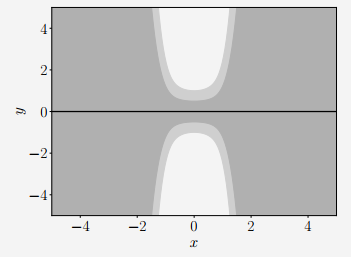
\includegraphics{graph15}
\end{center}
Shaded area is the distribution of the function and the black line is the mean function.
\begin{center}
	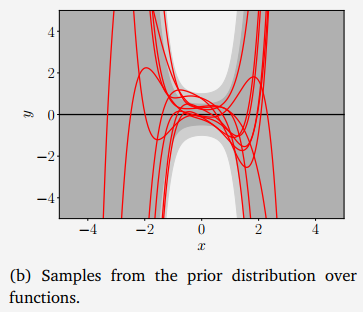
\includegraphics{graph16}
\end{center}
\subsubsection{Posterior Predictions}
Similar to prior predictions, we can also make posterior predations. Before making predictions using posterior distribution, we will first derive the posterior distribution. Given training inputs $x_n \in \mathbb{R}^D$ outputs $y_n \in \mathbb{R}$ $n=1, 2, 3,\dots, N$. Posterior over parameters($\theta$)
\begin{equation*}
	p(\theta|X, Y) = \frac{p(Y|X, \theta)p(\theta)}{p(Y|X)}.
\end{equation*}
Here, $X$ is the training set, $Y$ is corresponding training targets, $p(Y|X, \theta)$ is the likelihood and $p(\theta)$ is the prior.
\begin{align} \label{marginal}
	p(Y|X) &= \int p(Y|X, \theta)p(\theta)d\theta= E_\theta[p(Y|X, \theta)] 
\end{align}
is the marginal likelihood which is independent of $\theta$ and ensures that posterior is normalized($i.e.$ it integrates to $1$).
\begin{align*}
	p(Y|X, \theta) &= \mathcal{N}(y|\phi(x)\theta, \sigma^2I)
	\end{align*}
	This implies
	\begin{align*}
	p(\theta) &= \mathcal{N}(\theta|m_o, S_o) 
\end{align*}
As we know that $p(Y|X)$ is independent of $\theta$ we can ignore it. Our main aim is to find the posterior distribution
\begin{equation*}
	p(\theta|X, Y) = \mathcal{N}(\theta|m_N, S_N)
\end{equation*}
So we have to find these $m_N$ and $S_N$. The sum of log-prior and log-likelihood.
\begin{equation*}
	\log \mathcal{N}(y|\Phi\theta, \sigma^2I) + \log \mathcal{N}(\theta| m_o, S_o) = \frac{-1}{2}(\frac{(y-\Phi\theta)^T(y-\Phi\theta)}{\sigma^2} + (\theta - m_o)^TS_o^{-1}(\theta - m_o)) +const
\end{equation*}
 Here, constant represents the terms independent of $\theta$.
 \begin{align*}
 	\log \mathcal{N}(y|\Phi\theta, \sigma^2I) + \log \mathcal{N}(\theta| m_o, S_o) &= \frac{-1}{2}\big(\frac{y^Ty}{\sigma^2} - \frac{2y^T\Phi\theta}{\sigma^2} + \frac{\theta^T\Phi^T\Phi\theta}{\sigma^2}\\
 	&~~~~~~~~~~~~~ + \theta^TS_o^{-1}\theta - 2m_o^TS_o^{-1}\theta + m_o^TS_o^{-1}m_o\big)\\
 	&= \frac{-1}{2}(\theta^T(\sigma^{-2}\Phi^T\Phi + S_o^{-1})\theta - 2(\sigma^{-2}\Phi^Ty + S_o^{-1}m_o)^T\theta)
 \end{align*}
Now log-posterior 
\begin{align*}
	\log \mathcal{N}(\theta|m_N, S_N) &= \frac{-(\theta - m_N)^TS_N^{-1}(\theta - m_N)}{2} + const\\
	&= \frac{-(\theta^TS_N^{-1}\theta - 2m_N^TS_N^{-1}\theta + m_N^TS_N^{-1}m_N)}{2} + const\\
	&= \frac{-(\theta^TS_N^{-1}\theta -  2m_N^TS_N^{-1}\theta)}{2} + \text{constant}.
\end{align*}
Now comparing linear and quadratic terms the above equations.
\begin{align*}
	S_N^{-1} &= \Phi^T\sigma^{-2}I\Phi + S_o^{-1}\\
	S_N &= (\sigma^{-2}\Phi^T\Phi + S_o^{-1})^{-1}
\end{align*}
and
\begin{align*}
	m_N^TS_N^{-1} &= (\sigma^{-2}\Phi^Ty + S_o^{-1}m_o)^T\\
	m_N &= S_N(\sigma^{-2}\Phi^Ty + S_o^{-1}m_o)
\end{align*}
Now that we have calculated the posterior distribution.
$$p(\theta|X, Y) = \mathcal{N}(\theta|m_N, S_N).$$
Hence, we can now make predictions using posterior distribution. This is very similar to the prior predictions.
\begin{align*}
	p(y_*| X, Y, x_*) &= \int p(y_*|x_*, \theta)p(\theta|X, Y)d\theta\\
	&= \int \mathcal{N}(y_*|\phi^T(x_*)\theta, \sigma^2)\mathcal{N}(\theta|m_N, S_N)d\theta\\
	&= \mathcal{N}(y_*| \phi^T(x_*)m_N, \phi^T(x_*)S_N\phi(x_*) + \sigma^2)
\end{align*}
Here we see that the predictive mean is $\phi^T(x_*)m_N$. We can see that
\begin{equation*}
	p(y_*|X, Y, x_*) = E_{\theta|X,Y}[p(y_*|x_*, \theta)]
\end{equation*}
where it is the expectation of $p(y_*|x_*, \theta)$ with respect to parameter posterior $p(\theta|X, Y)$. We see that we have find out the distribution $p(y_*|X, Y, x_*)$. But if we want to find out the distribution of $f(x_*) = \phi^T(x)\theta$. We see that $f(x_*)$ will be noise-free. Hence,we will see that only the $\sigma^2$ will be committed in the expression. We obtain
\begin{equation*}
	p(y_*| X, Y, x_*) = \mathcal{N}(y_*| \phi^T(x_*)m_N, \phi^T(x_*)S_N\phi(x_*) + \sigma^2)
\end{equation*}
Now \begin{align*}
	E[f(x_*)|X, Y] &= E[\phi^T(x_*)\phi|X, Y]= \phi^T(x_*)E[\theta|X, Y]= \phi^T(x_*)m_N
\end{align*}
and
\begin{align*}
	Var[f(x_*)|X, Y] &= Var[\phi^T(x_*)\theta|X, Y]= \phi^T(x_*)Var[\theta|X, Y]\phi(x_*)= \phi^T(x_*)S_N\phi(x_*)
\end{align*}
Therefore,
\begin{equation*}
f(x_*) = \mathcal{N}(\phi^T(x_*)m_N, \phi^T(x_*)S_N\phi(x_*))
\end{equation*}
We see that the mean function will be $\phi^T(x)m_N$ which will coincide with the MAP estimate.

\vskip 1ex
\noindent
\textbf{Example}. Suppose this is the training data
\begin{center}
	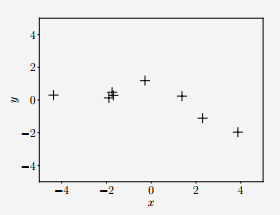
\includegraphics[height=7cm]{graph17}
\end{center}
Now consider this graph:
\begin{center}
	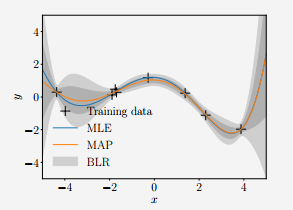
\includegraphics[height=7cm]{graph18}
\end{center}
Shaded area represents the distribution of the functions. Also the mean of this distribution will correspond to the MAP estimate curve. Now, consider the following graphs \\
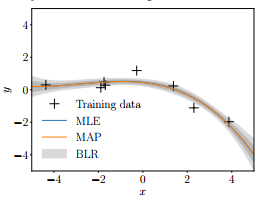
\includegraphics[scale=0.9]{graph19}
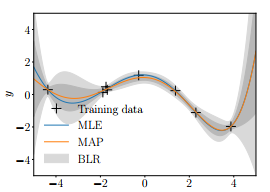
\includegraphics[scale=0.9]{graph20}
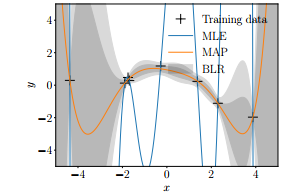
\includegraphics[scale=0.9]{graph21}
The first graph is for the polynomial of degree 3, the second graph is for polynomial of degree 5 and third is for degree 7. From these graphs, we can clearly see that as the polynomial degree increases the posterior uncertainty increases rapidly. Hence, we can conclude that the BLR(Bayesian Linear Regression) can help us to find the extent to which the uncertainty will occur in making predictions from the MAP estimate as the MAP estimate is the mean of the posterior distribution. Hence, if we are given a training data and we need to fit a function to it
\begin{enumerate}
	\item Then we can start by using MLE estimate to get some sort of unregularized function to it.
	\item Then we can go with MAP estimate to regularize the MLE estimate.
	\item Then we can go with BLR to compare the uncertainity between different models and get the distribution over functions.
\end{enumerate}
\subsection{Marginal Likelihood}
We saw in Bayesian linear regression while making posterior predictions \textbf{(\ref{marginal})} that $p(Y|X)$ is called the marginal likelohood, and it is used to normalize $p(\theta|X, Y)$ .
\begin{equation*}
	p(\theta|X, Y) = \frac{p(Y|X, \theta)p(\theta)}{p(Y|X)}
\end{equation*}
and
\begin{align*} 
	p(Y|X) &= \int p(Y|X, \theta)p(\theta)d\theta\\ 
	&= E_\theta[p(Y|X, \theta)]
\end{align*}
Hence, the marginal likelihood can be interpreted as the average value of likelihood $p(Y|X, \theta)$ for all the plausible values of $\theta$ over the prior. Now, the given model is 
\begin{align*}
	p(\theta) =  \mathcal{N}(m_o, S_o)\\
	p(Y|X, \theta) = \mathcal{N}(X\theta, \sigma^2I)
\end{align*}
Hence, solving the above equations we get the marginal likelihood as 
\begin{equation*}
	p(Y|X) = \mathcal{N}(y|Xm_o, XS_oX^T + \sigma^2I)
\end{equation*}
\subsection{Maximum Likelihood As Orthogonal Projection}
Given the noisy dataset
\begin{center}
	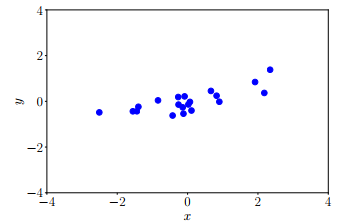
\includegraphics{graph22}
\end{center}
We can fit a line to this data by finding out $\theta_{ML} = (X^TX)^{-1}X^Ty$. During our derivation of this formula we aimed at maximizing the squared errors. Geometrically, we can see that
\begin{center}
	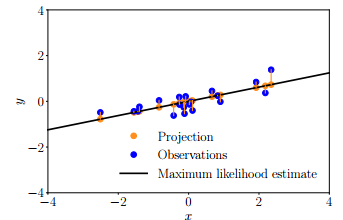
\includegraphics{graph23}
\end{center}
We have to minimize the orthogonal projection of the given data onto the line.
\section{Main Results}
An insurance company has the dataset of the charges they charge for their insurance for a person considering the following features:
\begin{enumerate}
	\item Age 
	\item Sex
	\item BMI
	\item Number of Children
	\item If he/she is a smoker
	\item Region
\end{enumerate}
Link for the dataset - \href{https://www.kaggle.com/mirichoi0218/insurance}{\textit{\textcolor{blue}{Insurance Datset}}}. So we have to train a regression model to predict the insurance price for a new person given his/her data.\\
\textbf{\large{Importing the required libraries}}
\begin{lstlisting}[language=Python]
	import numpy as np
	import pandas as pd
	import matplotlib.pyplot as plt
	from scipy.stats import pearsonr
\end{lstlisting}
\textbf{\large{Loading the Dataset}}
\begin{lstlisting}
	df=pd.read_csv('insurance.csv')
	df.head()
\end{lstlisting}
\begin{center}
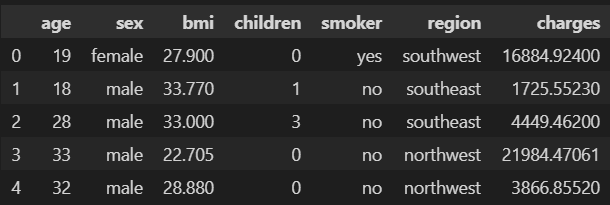
\includegraphics[width=8cm]{work1}
\end{center}
Let us analyse the effect of Age on Charges\\
\textbf{\large{Age Vs Charges}}
\begin{lstlisting}
	plt.scatter(df['age'], df['charges'])
	plt.ylabel('Charges')
	plt.xlabel('Age')
	plt.title('Age vs Charges')
\end{lstlisting}
\begin{center}
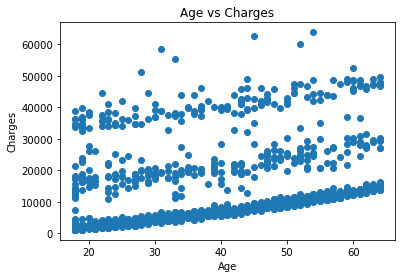
\includegraphics[width=8cm]{work2}
\end{center}
\begin{lstlisting}
	corr, _ = pearsonr(df['age'],df['charges'])
	print("Correlation between AGE and CHARGES ---> ", corr)
\end{lstlisting}
\begin{center}

\includegraphics[width=8cm]{work3}
\end{center}
We can see that the graph is divided into 3 parts. Let us see the effect of smoker and non-smoker on the same graph.
\begin{lstlisting}
	colors={'yes':'red','no':'blue'}
	plt.scatter(df['age'], df['charges'],c=df['smoker'].map(colors))
	plt.ylabel('Charges')
	plt.xlabel('Age')
	plt.title('Age vs Charges')
	plt.text(x=70, y=50000,s='Red:Smoker      Blue:Non-Smoker', fontsize=16)
\end{lstlisting}
\begin{center}
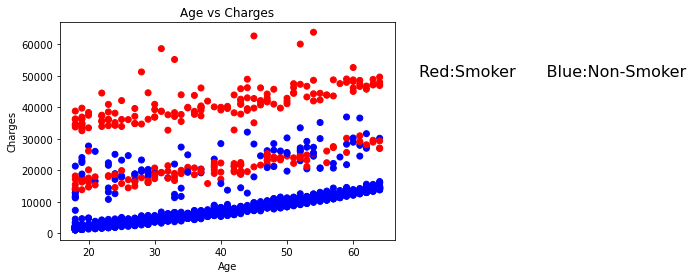
\includegraphics[width=8cm]{work4}
\end{center}
Hence we can see that we can segregate the data for smoker and non-smoker and train different models on both. Before segregating the data let us define the functions for the models that we will use to train using the results from the literature survey.
\begin{lstlisting}
	def model(x,Y, regularization=0, power=1):
		X=np.ones(x.shape[0])
		temp=np.ones(x.shape[0])
		for i in range(power):
			temp=temp*x
			X=np.c_[X,temp]
		theta=np.dot(np.dot(np.linalg.inv(np.dot(X.T,X)+regularization),X.T),Y)
		Y_pred=np.dot(X,theta)
		loss=np.sum(np.square(Y-Y_pred))/x.shape[0] + regularization*np.sum(np.square(theta))
		return theta,Y_pred,loss
\end{lstlisting}
\begin{lstlisting}
	def model1(x,Y, regularization=0, power=1):
		temp=np.ones(x.shape[0])
		X=np.c_[x,temp]
		theta=np.dot(np.dot(np.linalg.inv(np.dot(X.T,X)+regularization),X.T),Y)
		Y_pred=np.dot(X,theta)
		loss=np.sum(np.square(Y-Y_pred))/x.shape[0] + regularization*np.sum(np.square(theta))
		return theta,Y_pred,loss
\end{lstlisting}
\begin{lstlisting}
	def graph(x,Y,power,df_smoker):
		theta, Y_pred, loss=model(x,Y,regularization=0,power=power)
		plt.scatter(df_smoker['age'], df_smoker['charges'])
		plt.plot(x,Y_pred,'r+')
		plt.ylabel('Charges')
		plt.xlabel('Age')
		plt.title('Age vs Charges')
		print('loss = ',loss)
\end{lstlisting}
\textbf{\large{Smokers}}
\begin{lstlisting}
	df_smoker=df[df['smoker']=='yes']
	x=df_smoker['age'].to_numpy()
	Y=df_smoker['charges'].to_numpy()
\end{lstlisting}
\begin{lstlisting}
	corr, _ = pearsonr(df_smoker['age'],df_smoker['charges'])
	print("Correlation b/w AGE and CHARGES for smokers", corr)
\end{lstlisting}
\begin{center}

\includegraphics[width=8cm]{work5}
\end{center}
Applying the model on the smokers dataset
\begin{lstlisting}
	graph(x,Y,10,df_smoker)
\end{lstlisting}
\begin{center}
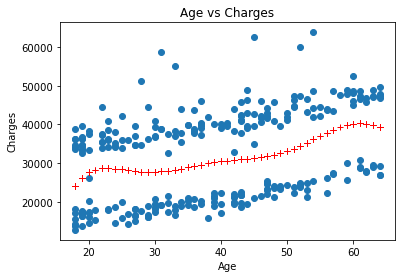
\includegraphics[width=6cm]{work6}
\end{center}
We see that our graph is still distributed into two parts. So we can segregate it more by dividing it into two parts -
\begin{enumerate}
	\item People with BMI<=30
	\item People with BMI>30
\end{enumerate}
\begin{lstlisting}
	df_smoker_high=df_smoker[df_smoker['bmi']>30]
	df_smoker_low=df_smoker[df_smoker['bmi']<=30]
\end{lstlisting}
\textbf{\large{Smokers with BMI>30}}
\begin{lstlisting}
	plt.scatter(df_smoker_high['age'], df_smoker_high['charges'])
	plt.ylabel('Charges')
	plt.xlabel('Age')
	plt.title('Age vs Charges For Smokers with BMI>30')
\end{lstlisting}
\begin{center}
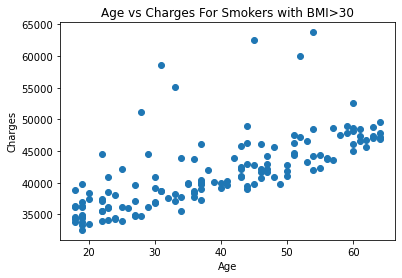
\includegraphics[width=8cm]{work7}
\end{center}
We can see that this is a good distribution for our linear regression model. We can improve a bit by removing the points with charges >50,000. This will improve our model.
\begin{lstlisting}
	df_smoker_high=df_smoker_high[df_smoker_high['charges']<=50000]
	plt.scatter(df_smoker_high['age'], df_smoker_high['charges'])
	plt.ylabel('Charges')
	plt.xlabel('Age')
	plt.title('Age vs Charges For Smokers with BMI>30')
\end{lstlisting}
\begin{center}
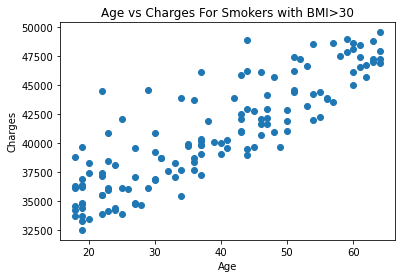
\includegraphics[width=7cm]{work8}
\end{center}
\begin{lstlisting}
	corr, _ = pearsonr(df_smoker_high['age'],df_smoker_high['charges'])
	print("Correlation b/w AGE and CHARGES", corr)
\end{lstlisting}
\begin{center}

\includegraphics[width=7cm]{work9}
\end{center}
We can see that we are having a high correlation as compared to previous ones. Now, training the model for smokers with BMI>30.
\begin{lstlisting}
	df_smoker_high=df_smoker_high.replace({'male':0, 'female':1, 'northwest':0, 'northeast':1, 'southwest':2, 'southeast':3})
	x=df_smoker_high.drop(columns=['charges','smoker']).to_numpy()
	Y=df_smoker_high['charges'].to_numpy()
	theta1,Y_pred,loss = model1(x,Y)
	xp=df_smoker_high['age'].to_numpy()
	plt.scatter(df_smoker_high['age'], df_smoker_high['charges'])
	plt.plot(xp,Y_pred,'r+')
	plt.ylabel('Charges')
	plt.xlabel('Age')
	plt.title('Age vs Charges For Smokers with BMI>30')
\end{lstlisting}
\begin{center}
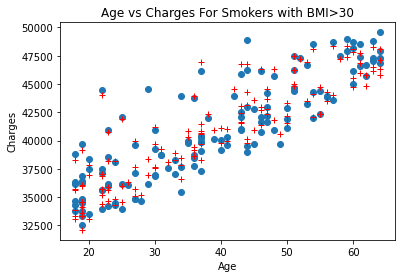
\includegraphics[width=7cm]{work10}\\
\end{center}
\textbf{\large{Smokers with BMI<=30}}
\begin{lstlisting}
	plt.scatter(df_smoker_low['age'], df_smoker_low['charges'])
	plt.ylabel('Charges')
	plt.xlabel('Age')
	plt.title('Age vs Charges For Smokers with BMI<=30')
\end{lstlisting}
\begin{center}
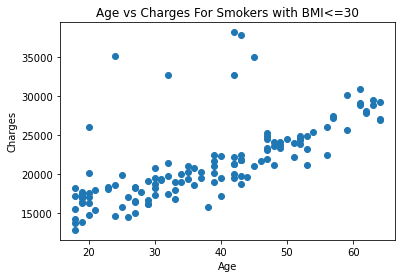
\includegraphics[width=7cm]{work11}\\
\end{center}
This is good but we can improve by putting an upper limit on charges i.e. 30,000.
\begin{lstlisting}
	df_smoker_low=df_smoker_low[df_smoker_low['charges']<=30000]
	plt.scatter(df_smoker_low['age'], df_smoker_low['charges'])
	plt.ylabel('Charges')
	plt.xlabel('Age')
	plt.title('Age vs Charges For Smokers with BMI<=30')
\end{lstlisting}
\begin{center}
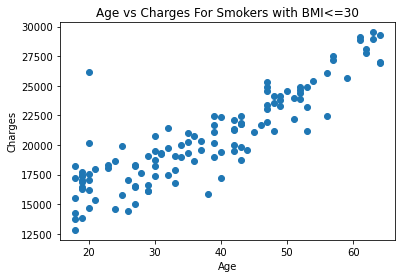
\includegraphics[width=7cm]{work12}
\end{center}
\begin{lstlisting}
	corr, _ = pearsonr(df_smoker_high['age'],df_smoker_high['charges'])
	print("Correlation b/w AGE and CHARGES", corr)
\end{lstlisting}
\begin{center}

\includegraphics[width=7cm]{work13}\\
\end{center}
We are having a good correlation, so we will train the model for this also..
\begin{lstlisting}
	df_smoker_low=df_smoker_low.replace({'male':0, 'female':1, 'northwest':0, 'northeast':1, 'southwest':2, 'southeast':3})
	x=df_smoker_low.drop(columns=['charges','smoker']).to_numpy()
	Y=df_smoker_low['charges'].to_numpy()
	theta2,Y_pred,loss = model1(x,Y)
	xp=df_smoker_low['age'].to_numpy()
	plt.scatter(df_smoker_low['age'], df_smoker_low['charges'])
	plt.plot(xp,Y_pred,'r+')
	plt.ylabel('Charges')
	plt.xlabel('Age')
	plt.title('Age vs Charges For Smokers with BMI<=30')
\end{lstlisting}
\begin{center}
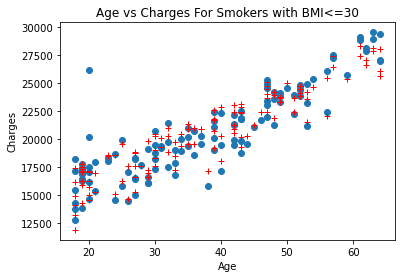
\includegraphics[width=7cm]{work14}
\end{center}
\textbf{\large{Non-Smokers}}
\begin{lstlisting}
	df_non_smoker=df[df['smoker']=='no']
	x=df_non_smoker['age'].to_numpy()
	Y=df_non_smoker['charges'].to_numpy()
	corr, _ = pearsonr(df_non_smoker['age'],df_non_smoker['charges'])
	print("Correlation b/w AGE and CHARGES for non-smokers", corr)
\end{lstlisting}
\begin{center}

\includegraphics[width=7cm]{work15}
\end{center}
\begin{lstlisting}
	graph(x,Y,8,df_non_smoker)
\end{lstlisting}
\begin{center}
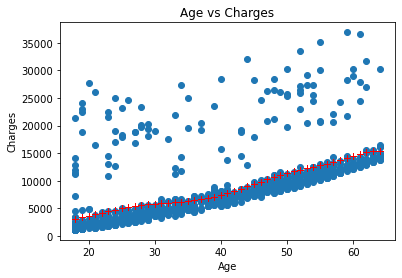
\includegraphics[width=7cm]{work16}
\end{center}
We see that though the model is fine but we can try to segregate it similarly using BMI..
\begin{lstlisting}
	df_non_smoker_high=df_non_smoker[df_non_smoker['bmi']>30]
	df_non_smoker_low=df_non_smoker[df_non_smoker['bmi']<=30]
\end{lstlisting}
\textbf{\large{Non-Smokers with BMI>30}}
\begin{lstlisting}
	plt.scatter(df_non_smoker_high['age'], df_non_smoker_high['charges'])
	plt.ylabel('Charges')
	plt.xlabel('Age')
	plt.title('Age vs Charges For Non-Smokers with BMI>30')
\end{lstlisting}
\begin{center}
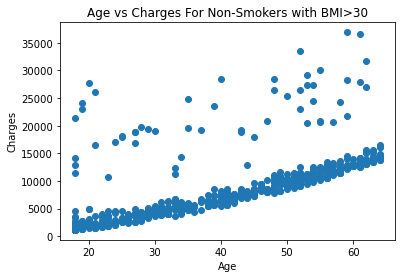
\includegraphics[width=7cm]{work17}
\end{center}
\textbf{\large{Non-Smokers with BMI<=30}}
\begin{lstlisting}
	plt.scatter(df_non_smoker_low['age'], df_non_smoker_low['charges'])
	plt.ylabel('Charges')
	plt.xlabel('Age')
	plt.title('Age vs Charges For Non-Smokers with BMI<=30')
\end{lstlisting}
\begin{center}
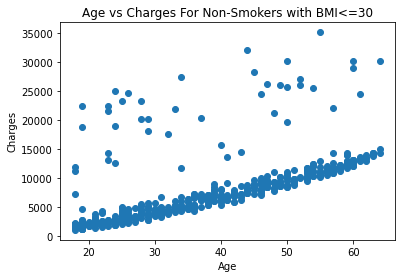
\includegraphics[width=7cm]{work18}
\end{center}
We see that we are unable to segregate the data on the basis of BMI.\\
So, lets put an upper bound of 16,000 on charges on the non-smoker dataset
\begin{lstlisting}
	df_non_smoker=df_non_smoker[df_non_smoker['charges']<=16000]
	plt.scatter(df_non_smoker['age'], df_non_smoker['charges'])
	plt.ylabel('Charges')
	plt.xlabel('Age')
	plt.title('Age vs Charges For Non-Smokers')
\end{lstlisting}
\begin{center}
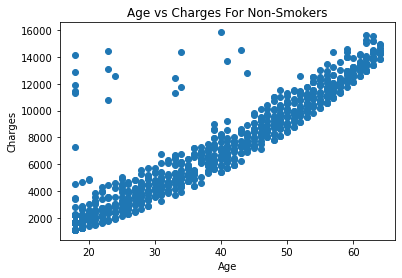
\includegraphics[width=7cm]{work19}
\end{center}
\begin{lstlisting}
	corr, _ = pearsonr(df_non_smoker['age'],df_non_smoker['charges'])
	print("Correlation b/w AGE and CHARGES for non-smokers", corr)
\end{lstlisting}
\begin{center}

\includegraphics[width=7cm]{work20}
\end{center}
High correlation means we can train a model for this.
\begin{lstlisting}
	df_non_smoker=df_non_smoker.replace({'male':0, 'female':1, 'northwest':0, 'northeast':1, 'southwest':2, 'southeast':3})
	x=df_non_smoker.drop(columns=['charges','smoker']).to_numpy()
	Y=df_non_smoker['charges'].to_numpy()
	theta3,Y_pred,loss = model1(x,Y)
	xp=df_non_smoker['age'].to_numpy()
	plt.scatter(df_non_smoker['age'], df_non_smoker['charges'])
	plt.plot(xp,Y_pred,'r+')
	plt.ylabel('Charges')
	plt.xlabel('Age')
	plt.title('Age vs Charges For Non-Smokers')
\end{lstlisting}
\begin{center}
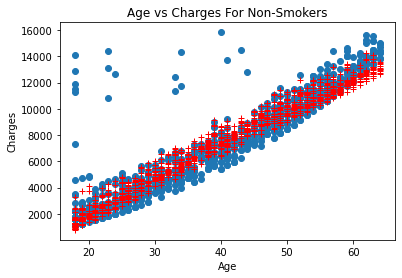
\includegraphics[width=7cm]{work21}
\end{center}
\textbf{\large{Making Predictions}}\\
For making predictions we will pass a numpy array to the following function with following entries in the mentioned order:
\begin{enumerate}
	\item Age
	\item $0$ if Male, $1$ is Female
	\item BMI
	\item Number of children
	\item $1$ if Smoker, $0$ if Non-Smoker
	\item Region: $0$ if NorthWest, $1$ if NorthEast, $2$ if SouthWest, $3$ if SouthEast 
\end{enumerate}
\begin{lstlisting}
	def predict(x):
		yp=[]
		x1=np.append(x,[1])
		x1=np.append(x1[:4],x1[5:])
		if x[4]==1:
			if x[2]>30:
				yp=np.dot(x1,theta1)
			else:
				yp=np.dot(x1,theta2)
		else:
			yp=np.dot(x1,theta3)
		return yp
\end{lstlisting}
\section{CONCLUSION}
Based on the understandings and results from the Literature Survey we trained a model that predicts the insurance price for a person given his Age, Sex, BMI, Number of Children, Smoking Status and Region. First, we analysed the dataset. The given data was too much scattered to be able to get a good model that fits it. So we segregated the data for smokers and non-smokers separately. Then we further segregated it using BMI. Still some scattered points were left due to unknown reasons of a particular person so we made a upper-bound to the data. This way we trained the model and finally we were able to get a decent result.
\end{document}



